\documentclass{report}
\title{APIO 2015 Problems}
\usepackage[margin=1in]{geometry}
\setlength{\parindent}{0pt}
\setlength{\parskip}{2pt}
\usepackage{graphicx}

\begin{document}
\maketitle

\newpage
\begin{center}
\section*{Bali Sculptures}
Time limit: 1 s\\
Memory limit: 64 MB
\end{center}

\subsection*{Description}

The province of Bali has many sculptures located on its roads. Let's focus on one of its main roads.

There are $N$ sculptures on that main road, conveniently numbered 1 through $N$ consecutively. The age of sculpture $i$ is $Y_{i}$ years. To make the road more beautiful, the government wants to partition the sculptures into several groups. Then, the government will plant beautiful trees between the groups, to attract more tourists to Bali.

Here is the rule in partitioning the sculptures:
\begin{itemize} \itemsep1pt \parskip0pt
\item The sculptures must be partitioned into exactly $X$ groups, where $A \le X \le B$. Each group must consist of at least one sculpture. Each sculpture must belong to exactly one group. The sculptures in each group must be consecutive sculptures on the road.
\item For each group, compute the sum of the ages of the sculptures in that group.
\item Finally, compute the bitwise OR of the above sums. Let's call this the final beauty value of the partition.
\end{itemize}

What is the minimum final beauty value that the government can achieve?

Note: the bitwise OR of two non-negative integers $P$ and $Q$ is computed as follows:

\begin{itemize} \itemsep1pt \parskip0pt
\item Convert $P$ and $Q$ into binary.
\item Let $nP$ = number of bits of $P$, and $nQ$ = number of bits of $Q$. Let $M = \max(nP, nQ)$.
\item Represent $P$ in binary as $p_{M-1}p_{M-2} .. p_1p_0$ and $Q$ in binary as $q_{M-1}q_{M-2} .. q_1q_0$, where $pi$ and $qi$ are the $i$-th bits of $p$ and $q$, respectively. The $(M-1)$st bits are the most significant bits, while the $0$th bits are the least significant bits.
\item $P$ OR $Q$, in binary, is defined as ($p_{M-1}$ OR $q_{M-1}$)($p_{M-2}$ OR $q_{M-2}$)..($p_1$ OR $q_1$)($p_0$ OR $q_0$), where
\begin{itemize} \itemsep1pt \parskip0pt
\item 0 OR 0 = 0
\item 0 OR 1 = 1
\item 1 OR 0 = 1
\item 1 OR 1 = 1
\end{itemize}
\end{itemize}

\subsection*{Input Format}
The first line contains three space-separated integers $N$, $A$, and $B$. The second line contains $N$ space-separated integers $Y_1, Y_2, ..., Y_N$.

\subsection*{Output Format}
A single line containing the minimum final beauty value.

\subsection*{Sample Input}
\begin{verbatim}
6 1 3
8 1 2 1 5 4
\end{verbatim}

\subsection*{Sample Output}
\begin{verbatim}
11
\end{verbatim}

\subsection*{Explanation}
Partition the sculptures into 2 groups: (8 1 2) and (1 5 4). The sums are (11) and (10). The final beauty value is (11 OR 10) = 11.

\subsection*{Subtasks}
\subsubsection{Subtask 1 (9 points)}
\begin{itemize} \itemsep1pt \parskip0pt
\item $1 \le N \le 20$
\item $1 \le A \le B \le N$
\item $0 \le Yi \le 1,000,000,000$
\end{itemize}

\subsubsection{Subtask 2 (16 points)}
\begin{itemize} \itemsep1pt \parskip0pt
\item $1 \le N \le 50$
\item $1 \le A \le B \le \min(20, N)$
\item $0 \le Y_i \le 10$
\end{itemize}

\subsubsection{Subtask 3 (21 points)}
\begin{itemize} \itemsep1pt \parskip0pt
\item $1 \le N \le 100$
\item $A = 1$
\item $1 \le B \le N$
\item $0 \le Y_i \le 20$
\end{itemize}

\subsubsection{Subtask 4 (25 points)}
\begin{itemize} \itemsep1pt \parskip0pt
\item $1 \le N \le 100$
\item $1 \le A \le B \le N$
\item $0 \le Y_i \le 1,000,000,000$
\end{itemize}

\subsubsection{Subtask 5 (29 points)}
\begin{itemize} \itemsep1pt \parskip0pt
\item $1 \le N \le 2,000$
\item $A = 1$
\item $1 \le B \le N$
\item $0 \le Y_i \le 1,000,000,000$
\end{itemize}

\newpage
\begin{center}
\section*{Jakarta Skyscrapers}
Time limit: 1 s\\
Memory limit: 256 MB
\end{center}

\subsection*{Description}

The city of Jakarta has $N$ skyscrapers located on a line, conveniently numbered 0 through $N$-1 from left to right. There are no other skyscrapers in Jakarta.

Jakarta is inhabited by $M$ mystical creatures called "\textbf{doge}"s. The doges are conveniently numbered 0 through $M$-1. Doge $i$ initially resides in skyscraper $B_i$. Doge $i$ has a mystical power, represented with a positive integer $P_i$. This mystical power enables doges to jump between skyscrapers. In a single jump, a doge with superpower $p$ that is currently in skyscraper $b$ can move to either skyscraper $b$+$p$ (if $0 \le b+p < N$) or skyscraper $b$-$p$ (if $0 \le b-p < N$).

Doge 0 is the most awesome doge, and it is the leader of all the doges. It has an urgent news for doge 1, and wants the news to reach doge 1 as quickly as possible. Any doge that has received the news can do any of the following actions:

\begin{itemize} \parskip0pt \itemsep1pt
\item Make a jump to move to some other skyscraper.
\item Pass the news to another doge in the same skyscraper.
\end{itemize}

Please help the doges by calculating the minimum number of total jumps required by all doges to pass the news to doge 1, or if it is impossible to do so.

\subsection*{Input Format}
The first line contains two integers $N$ and $M$. Each of the next $M$ lines contains two integers $B_i$ and $P_i$.

\subsection*{Output Format}
A single line containing the minimum number of total jumps, or -1 if it is impossible.

\subsection*{Sample Input}
\begin{verbatim}
5 3
0 2
1 1
4 1
\end{verbatim}

\subsection*{Sample Output}
\begin{verbatim}
5
\end{verbatim}

\subsection*{Explanation}
Here is one of the possible scenarios to pass the news using 5 jumps:
\begin{itemize} \itemsep1pt \parskip0pt
\item Doge 0 jumps to skyscraper 2 and then to skyscraper 4 (2 jumps).
\item Doge 0 passes the news to doge 2.
\item Doge 2 jumps to skyscraper 3, and then to skyscraper 2, and then to skyscraper 1 (3 jumps).
\item Doge 2 passes the news to doge 1.
\end{itemize}

\subsection*{Subtasks}

For each subtask,
\begin{itemize}
\item $0 \le B_i < N$
\end{itemize}

\subsubsection{Subtask 1 (10 points)}
\begin{itemize} \itemsep1pt \parskip0pt
\item $1 \le N \le 10$
\item $1 \le P_i \le 10$
\item $2 \le M \le 3$
\end{itemize}

\subsubsection{Subtask 2 (12 points)}
\begin{itemize} \itemsep1pt \parskip0pt
\item $1 \le N \le 100$
\item $1 \le P_i \le 100$
\item $2 \le M \le 2,000$
\end{itemize}

\subsubsection{Subtask 3 (14 points)}
\begin{itemize} \itemsep1pt \parskip0pt
\item $1 \le N \le 2,000$
\item $1 \le P_i \le 2,000$
\item $2 \le M \le 2,000$
\end{itemize}

\subsubsection{Subtask 4 (21 points)}
\begin{itemize} \itemsep1pt \parskip0pt
\item $1 \le N \le 2,000$
\item $1 \le P_i \le 2,000$
\item $2 \le M \le 30,000$
\end{itemize}

\subsubsection{Subtask 5 (43 points)}
\begin{itemize} \itemsep1pt \parskip0pt
\item $1 \le N \le 30,000$
\item $1 \le P_i \le 30,000$
\item $2 \le M \le 30,000$
\end{itemize}

\newpage
\begin{center}
\section*{Palembang Bridges}
Time limit: 2 s\\
Memory limit: 256 MB
\end{center}

\subsection*{Description}
\indent

The city of Palembang is separated by Musi River into two zones. Let's call them zone A and zone B.

Each zone consists of exactly 1,000,000,001 buildings along the respective side of the river, conveniently numbered 0 through 1,000,000,000. The distance between every pair of adjacent buildings is 1 unit of distance. The width of the river is 1 unit of distance as well. Building i in zone A is located on exactly the opposite side of building i in zone B.

$N$ citizens live and work in the city. Citizen i's house is in zone $P_i$, building $S_i$, while his office is in zone $Q_i$, building $T_i$. If a citizen must cross the river to go from his house to his office, he must take a boat. This has been uncomfortable, so the government has decided to build at most $K$ bridges over the river, so that the citizens can go to work by driving. Each bridge must be built exactly between two opposite buildings in the two zones. The bridges must be strictly perpendicular to the river. The bridges must not overlap each other.

Let $D_i$ be the minimum distance citizen i has to drive to go from his house to his office, after the government has built at most $K$ bridges. Help the government build the bridges in such a way that the sum $D_1 + D_2 + ... + D_N$ is minimized.

\subsection*{Input Format}
The first line contains two integers $K$ and $N$. Each of the next $N$ lines contains four tokens $P_i$, $S_i$, $Q_i$, and $T_i$.

\subsection*{Output Format}
A single line containing the minimum sum of the distances.

\subsection*{Sample Input 1}
\begin{verbatim}
1 5
B 0 A 4
B 1 B 3
A 5 B 7
B 2 A 6
B 1 A 7
\end{verbatim}

\subsection*{Sample Output 1}
\begin{verbatim}
24
\end{verbatim}

\subsection*{Sample Input 2}
\begin{verbatim}
2 5
B 0 A 4
B 1 B 3
A 5 B 7
B 2 A 6
B 1 A 7
\end{verbatim}

\subsection*{Sample Output 2}
\begin{verbatim}
22
\end{verbatim}

\subsection*{Explanation}
This is the illustration for both sample inputs.

\begin{center}
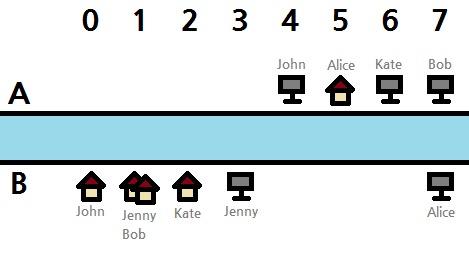
\includegraphics{images/bridge_initial}
\end{center}

Here is one possible solution for sample input 1. The pink stripe segment denotes a bridge.

\begin{center}
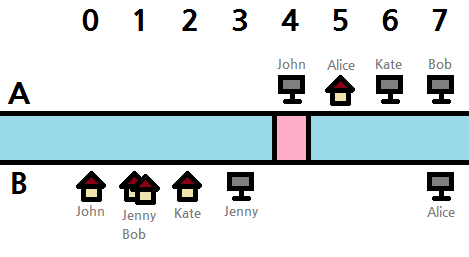
\includegraphics{images/bridge_1}
\end{center}

And this is a possible solution for sample input 2:

\begin{center}
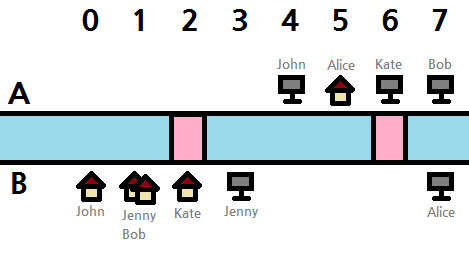
\includegraphics{images/bridge_2}
\end{center}
\subsection*{Subtasks}
For each subtask,
\begin{itemize} \parskip0pt \itemsep1pt
\item $P_i$ and $Q_i$ will be either a character 'A' or a character 'B'.
\item $0 \le S_i, T_i \le 1,000,000,000$
\item More than one house or office (or combination of both) can be located in the same building.
\end{itemize}

\subsubsection{Subtask 1 (8 points)}
\begin{itemize} \itemsep1pt \parskip0pt
\item $K = 1$
\item $1 \le N \le 1,000$
\end{itemize}

\subsubsection{Subtask 2 (14 points)}
\begin{itemize} \itemsep1pt \parskip0pt
\item $K = 1$
\item $1 \le N \le 100,000$
\end{itemize}

\subsubsection{Subtask 3 (9 points)}
\begin{itemize} \itemsep1pt \parskip0pt
\item $K = 2$
\item $1 \le N \le 100$
\end{itemize}

\subsubsection{Subtask 4 (32 points)}
\begin{itemize} \itemsep1pt \parskip0pt
\item $K = 2$
\item $1 \le N \le 1,000$
\end{itemize}

\subsubsection{Subtask 5 (37 points)}
\begin{itemize} \itemsep1pt \parskip0pt
\item $K = 2$
\item $1 \le N \le 100,000$
\end{itemize}

\end{document}
